\documentclass[11pt,a4paper]{article}
\usepackage[margin=18mm,top=22mm,bottom=20mm]{geometry}
\usepackage{fontspec}\setmainfont{Latin Modern Roman}
\usepackage{xcolor}\usepackage{amsmath,amssymb,tikz,graphicx,fancyhdr,array,needspace}
\usetikzlibrary{patterns,arrows.meta,decorations.pathmorphing,calc}
\setlength{\headheight}{14pt}
\usetikzlibrary{arrows.meta}
\pagestyle{fancy}\fancyhf{}\renewcommand{\headrulewidth}{0.4pt}
\fancyhead[L]{\textbf{M-10}}\fancyhead[C]{\itshape Fizika — yechimlar (OliyFizika.uz)}\fancyhead[R]{\textbf{Mock №10}}
\fancyfoot[C]{\thepage}
\setlength{\parindent}{0pt}\setlength{\parskip}{3pt}
\newcommand{\opt}[2]{\hspace*{4mm}#1)\ #2\par}
\newcommand{\blank}{\rule{5cm}{0.4pt}}
\begin{document}

\begin{center}{\Large\textbf{FIZIKA — YECHIMLAR}}\\[2pt]{\large Mock №10}\end{center}
\Needspace{10\baselineskip}\noindent\begin{minipage}{\linewidth}
\textbf{1.}\ Ikkita avtomobil $x_1=5t+0{,}2t^2$ [m] va $x_2=24-4t$ [m] qonuniyatlar bilan harakatlanmoqda. Ikkinçi avtomobil $x_2=0$ koordinataga yetib borganda birinçi avtomobil qaysi koordinataga yetib boradi (m)?\par\smallskip
\opt{A}{37}
\opt{B}{37,2}
\opt{C}{38}
\opt{D}{40}
\end{minipage}\vspace{2pt}\par
\noindent\colorbox{gray!12}{\parbox{\dimexpr\linewidth-2\fboxsep}{\textbf{Javob: B) 37,2}}}\par\smallskip
\noindent\textit{Yechim.}\ $x_2=0$ bölganda $24-4t=0$, $t=6$ s. Şu paytda $x_1=5\cdot6+0{,}2\cdot36=30+7{,}2=37{,}2$ m.\par\par\medskip\hrule\medskip
\Needspace{10\baselineskip}\noindent\begin{minipage}{\linewidth}
\textbf{2.}\ 1 kg massali jism suvda qanday tezlaniş bilan çökadi (m/s$^{2}$). $\rho$suv =1000 kg/m$^{3}$, $\rho$jism =4000 kg/m$^{3}$. g=10 N/kg.\par\smallskip
\opt{A}{7,5}
\opt{B}{8}
\opt{C}{6}
\opt{D}{10}
\end{minipage}\vspace{2pt}\par
\noindent\colorbox{gray!12}{\parbox{\dimexpr\linewidth-2\fboxsep}{\textbf{Javob: A) 7,5}}}\par\smallskip
\noindent\textit{Yechim.}\ $ma=mg-\rho_s gV$, $V=m/\rho$:\par
\[a=g\left(1-\frac{\rho_s}{\rho}\right)=10\left(1-\frac{1000}{4000}\right)=7{,}5\ \text{m/s}^2.\]\par\medskip\hrule\medskip
\Needspace{10\baselineskip}\noindent\begin{minipage}{\linewidth}
\textbf{3.}\ Ziçligi 300 kg/m$^{3}$ bölgan 0,1 m$^{3}$ hajmli pökak suvda suzmoqda. Uning ustiga qanday massali (kg) jism qöyilsa, pökak umumiy hajmining 1/4 qismi suv ustida qoladi. $\rho_{suv}$=1000 kg/m$^{3}$\par\smallskip
\opt{A}{45}
\opt{B}{15}
\opt{C}{60}
\opt{D}{30}
\end{minipage}\vspace{2pt}\par
\noindent\colorbox{gray!12}{\parbox{\dimexpr\linewidth-2\fboxsep}{\textbf{Javob: A) 45}}}\par\smallskip
\noindent\textit{Yechim.}\ Pökakning $3/4$ qismi botgan: Arximed kuçi $1000\cdot0{,}075\cdot g$, ya’ni $75$ kg li jism oğirligini kötaradi. Pökak massasi $300\cdot0{,}1=30$ kg, yuk $75-30=45$ kg.\par\par\medskip\hrule\medskip
\Needspace{10\baselineskip}\noindent\begin{minipage}{\linewidth}
\textbf{4.}\ Jismga 69 N va 74 N kuçlar qöyilgan. Bu kuçlarning natijavyisi 5 N bölsa, ular orasidagi burçakni aniqlang.\par\smallskip
\opt{A}{90$^\circ$}
\opt{B}{150$^\circ$}
\opt{C}{180$^\circ$}
\opt{D}{60$^\circ$}
\end{minipage}\vspace{2pt}\par
\noindent\colorbox{gray!12}{\parbox{\dimexpr\linewidth-2\fboxsep}{\textbf{Javob: C) 180$^\circ$}}}\par\smallskip
\noindent\textit{Yechim.}\ Natijaviy kuç $74-69=5$ N — kuçlarning ayirmasiga teng, demak ular qarama-qarşi yönalgan: $180^\circ$.\par\par\medskip\hrule\medskip
\Needspace{10\baselineskip}\noindent\begin{minipage}{\linewidth}
\textbf{5.}\ Poyezd şarqqa qarab yerga nisbatan (80 km/h) tekis harakatlanmoqda. Osmonda uçayotgan samolyotdagi (900 km/h) passajirga poyezd huddi ğarbga ketayotgandek körinsa, samolyot qaysi yönalişda uçayotgan böladi?\par\smallskip
\opt{A}{şarqqa}
\opt{B}{ğarbga}
\opt{C}{janubga}
\opt{D}{şimolga}
\end{minipage}\vspace{2pt}\par
\noindent\colorbox{gray!12}{\parbox{\dimexpr\linewidth-2\fboxsep}{\textbf{Javob: A) şarqqa}}}\par\smallskip
\noindent\textit{Yechim.}\ Samolyot şarqqa poyezddan tezroq uçsa ($900>80$), samolyotga nisbatan poyezd ğarbga ketayotgandek körinadi.\par\par\medskip\hrule\medskip
\Needspace{10\baselineskip}\noindent\begin{minipage}{\linewidth}
\textbf{6.}\ $\upsilon$ $\ge$12 m/s tezlik bilan yuqoriga tik otilgan jismning kötarilişning oxirgi sekundidagi örtaça tezligini (m/s) aniqlang. g=10 m/s$^{2}$.\par\smallskip
\opt{A}{6}
\opt{B}{5}
\opt{C}{7}
\opt{D}{8}
\end{minipage}\vspace{2pt}\par
\noindent\colorbox{gray!12}{\parbox{\dimexpr\linewidth-2\fboxsep}{\textbf{Javob: B) 5}}}\par\smallskip
\noindent\textit{Yechim.}\ Kötarilişning oxirgi sekundi — eng yuqori nuqtagaça qolgan 1 s. Teskari qaraganda bu erkin tuşişning birinçi sekundi: $s=g\cdot1^2/2=5$ m, örtaça tezlik $5$ m/s.\par\par\medskip\hrule\medskip
\Needspace{10\baselineskip}\noindent\begin{minipage}{\linewidth}
\textbf{7.}\ Ikkita mayatnik rasmda körsatilganidek muvozanat nuqtasidan çiqarilib qöyib yuborildi. Birinçisining tebraniş davri 2 s, ikkinçisiniki 3 s. Tebraniş boşlanganda ularning dastlabki vaziyati rasmda körsatilganidek bölgan deb tasavvur qilib, 50 s da ular neça marta dastlabki vaziyatga kelişini hisoblang.\par\smallskip
\noindent\hspace*{4mm}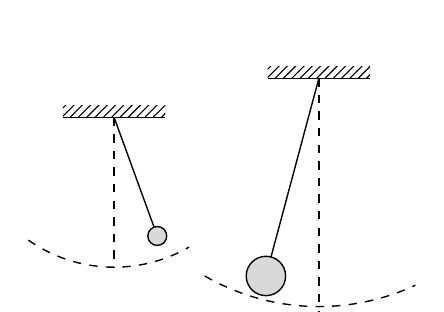
\begin{tikzpicture}[x=1cm,y=1cm,line width=0.5pt,>=Stealth,font=\small]
\fill[pattern=north east lines,draw=none] (0,3.0) rectangle (1.3,3.15); \draw (0,3.0)--(1.3,3.0);
\draw (0.65,3.0)--++(-70:1.6) coordinate(b1); \draw[dashed] (0.65,3.0)--++(0,-1.9);
\draw[fill=gray!30] (b1) circle(0.12);
\draw[dashed] (0.65,3.0)+(-125:1.9) arc(-125:-60:1.9);
\fill[pattern=north east lines,draw=none] (2.6,3.5) rectangle (3.9,3.65); \draw (2.6,3.5)--(3.9,3.5);
\draw (3.25,3.5)--++(-105:2.6) coordinate(b2); \draw[dashed] (3.25,3.5)--++(0,-3.1);
\draw[fill=gray!30] (b2) circle(0.25);
\draw[dashed] (3.25,3.5)+(-120:2.9) arc(-120:-65:2.9);
\end{tikzpicture}\par\smallskip
\opt{A}{6}
\opt{B}{8}
\opt{C}{4}
\opt{D}{13}
\end{minipage}\vspace{2pt}\par
\noindent\colorbox{gray!12}{\parbox{\dimexpr\linewidth-2\fboxsep}{\textbf{Javob: B) 8}}}\par\smallskip
\noindent\textit{Yechim.}\ Birinçi mayatnik dastlabki vaziyatiga har 2 s da, ikkinçisi har 3 s da qaytadi. Ikkalasi bir vaqtda dastlabki vaziyatda bölişi uçun $\mathrm{EKUK}(2;3)=6$ s kerak. 50 s içida: $6, 12, \ldots, 48$ — 8 marta.\par\par\medskip\hrule\medskip
\Needspace{10\baselineskip}\noindent\begin{minipage}{\linewidth}
\textbf{8.}\ Tabiati jihatidan qanday bölişidan qat’iy nazar, kuçlarning jismga bir vaqtdagi ta’siri uning tezligini özgartirmasa (ya’ni, unga tezlaniş bermasa), bu kuçlar......... yönalgan böladi.\par\smallskip
\opt{A}{moduli jihatidan teng va qarama-qarşi}
\opt{B}{moduli jihatidan teng va özaro tik}
\opt{C}{moduli jihatidan farq qiluvçi va qarama-qarşi}
\opt{D}{moduli jihatidan teng va bir xil}
\end{minipage}\vspace{2pt}\par
\noindent\colorbox{gray!12}{\parbox{\dimexpr\linewidth-2\fboxsep}{\textbf{Javob: A) moduli jihatidan teng va qarama-qarşi}}}\par\smallskip
\noindent\textit{Yechim.}\ Tezlaniş bölmasa, kuçlarning teng ta’sir etuvçisi nol: ikki kuç moduli teng va qarama-qarşi yönalgan.\par\par\medskip\hrule\medskip
\Needspace{10\baselineskip}\noindent\begin{minipage}{\linewidth}
\textbf{9.}\ 500 m balandlikdan 15 m/s tezlik bilan gorizontal otilgan jismning qança vaqtdan keyin tangensial va normal tezlanişlari tenglaşadi (s)?\par\smallskip
\opt{A}{3,0}
\opt{B}{1,5}
\opt{C}{2,5}
\opt{D}{4,5}
\end{minipage}\vspace{2pt}\par
\noindent\colorbox{gray!12}{\parbox{\dimexpr\linewidth-2\fboxsep}{\textbf{Javob: B) 1,5}}}\par\smallskip
\noindent\textit{Yechim.}\ Tangensial va normal tezlanişlar teng bölişi uçun tezlik vektori gorizont bilan $45^\circ$ hosil qilişi kerak: $v_y=v_x$, $gt=15$, $t=1{,}5$ s.\par\par\medskip\hrule\medskip
\Needspace{10\baselineskip}\noindent\begin{minipage}{\linewidth}
\textbf{10.}\ Jism 80 m balandlikdan erkin tuşmoqda. Uning massasi 6,4 kg ga teng. Jism yerga mutloq elastik urilgan bölsa, tuşiş boşlangandan 9 s dan keyin uning potensial energiyasi qançaga (J) teng böladi?\par\smallskip
\opt{A}{2400}
\opt{B}{5600}
\opt{C}{4800}
\opt{D}{7200}
\end{minipage}\vspace{2pt}\par
\noindent\colorbox{gray!12}{\parbox{\dimexpr\linewidth-2\fboxsep}{\textbf{Javob: C) 4800}}}\par\smallskip
\noindent\textit{Yechim.}\ Tuşiş vaqti $t=\sqrt{2h/g}=4$ s. Elastik urilişdan keyin jism 4 s da yana 80 m ga kötariladi (8 s). 9-sekundda u yana 1 s erkin tuşadi: $5$ m pastlaydi, $h=75$ m.\par
\[E_p=mgh=6{,}4\cdot10\cdot75=4800\ \text{J}.\]\par\medskip\hrule\medskip
\Needspace{10\baselineskip}\noindent\begin{minipage}{\linewidth}
\textbf{11.}\ Massasi 2 kg bölgan çöyan dazmol gaz öçoqda 20 $^\circ$C dan 240 $^\circ$C gaça qizdirildi. Gaz yonişida ajralgan barça issiqlik dazmolga berilgan deb, yoqilgan gaz massasi topilsin (g). Gazning soliştirma yoniş issiqligi 44 MJ/kg, çöyanning soliştirma issiqlik siğimi esa 540 J/kg$\cdot$K.\par\smallskip
\opt{A}{5,4}
\opt{B}{6,5}
\opt{C}{5,8}
\opt{D}{6}
\end{minipage}\vspace{2pt}\par
\noindent\colorbox{gray!12}{\parbox{\dimexpr\linewidth-2\fboxsep}{\textbf{Javob: A) 5,4}}}\par\smallskip
\noindent\textit{Yechim.}\ $Q=cm\Delta t=540\cdot2\cdot220=237\,600$ J; gaz massasi $m=\frac{Q}{q}=\frac{237\,600}{44\cdot10^6}=5{,}4\cdot10^{-3}$ kg $=5{,}4$ g.\par\par\medskip\hrule\medskip
\Needspace{10\baselineskip}\noindent\begin{minipage}{\linewidth}
\textbf{12.}\ Gazga 250 J issiqlik miqdori berildi. Gaz 120 J iş bajargan bölsa, uning içki energiyasi qanday özgargan?\par\smallskip
\opt{A}{130 J ga kamayadi}
\opt{B}{130 J ga ortadi}
\opt{C}{370 J ga ortadi}
\opt{D}{120 J ga kamayadi}
\end{minipage}\vspace{2pt}\par
\noindent\colorbox{gray!12}{\parbox{\dimexpr\linewidth-2\fboxsep}{\textbf{Javob: B) 130 J ga ortadi}}}\par\smallskip
\noindent\textit{Yechim.}\ $\Delta U=Q-A=250-120=130$ J — ortadi.\par\par\medskip\hrule\medskip
\Needspace{10\baselineskip}\noindent\begin{minipage}{\linewidth}
\textbf{13.}\ Temperaturalari 50 $^\circ$C va 10 $^\circ$C bölgan ikkita şarlar özaro tekkizildi va ularning temperaturalari 40 $^\circ$C bölib qoldi. Şarlarning soliştirma issiqlik siğimlari C$_{1}$ va C$_{2}$ bölsa, ularning nisbatini (C$_{1}$ /C$_{2}$) aniqlang.\par\smallskip
\opt{A}{1/3}
\opt{B}{2}
\opt{C}{3}
\opt{D}{1/2}
\end{minipage}\vspace{2pt}\par
\noindent\colorbox{gray!12}{\parbox{\dimexpr\linewidth-2\fboxsep}{\textbf{Javob: C) 3}}}\par\smallskip
\noindent\textit{Yechim.}\ Şarlar massalari teng deb: $c_1m(50-40)=c_2m(40-10)$, $c_1/c_2=3$.\par\par\medskip\hrule\medskip
\Needspace{10\baselineskip}\noindent\begin{minipage}{\linewidth}
\textbf{14.}\ Temperaturalari bir xil bölgan bir xil massali argon va geliyning içki energiyasini taqqoslang.\par\smallskip
\opt{A}{geliyniki 100 marta katta}
\opt{B}{geliyniki 10 marta kiçik}
\opt{C}{ikkalasi bir xil.}
\opt{D}{geliyniki 10 marta katta}
\end{minipage}\vspace{2pt}\par
\noindent\colorbox{gray!12}{\parbox{\dimexpr\linewidth-2\fboxsep}{\textbf{Javob: D) geliyniki 10 marta katta}}}\par\smallskip
\noindent\textit{Yechim.}\ Bir atomli gaz uçun $U=\frac32\frac{m}{M}RT$, ya’ni $U\sim1/M$. $M_{Ar}=40$, $M_{He}=4$ — geliyniki 10 marta katta.\par\par\medskip\hrule\medskip
\Needspace{10\baselineskip}\noindent\begin{minipage}{\linewidth}
\textbf{15.}\ 0 $^\circ$C da metall sterjen 10 m$^{3}$ hajmga ega. Uning 800 $^\circ$C dagi hajmini (m$^{3}$) toping. Sterjenning çiziqli kengayiş koeffitsiyenti $\alpha=1\cdot10^{-5}$ K$^{-1}$.\par\smallskip
\opt{A}{10,24}
\opt{B}{11}
\opt{C}{12}
\opt{D}{9}
\end{minipage}\vspace{2pt}\par
\noindent\colorbox{gray!12}{\parbox{\dimexpr\linewidth-2\fboxsep}{\textbf{Javob: A) 10,24}}}\par\smallskip
\noindent\textit{Yechim.}\ Hajmiy kengayiş koeffitsiyenti $\beta=3\alpha=3\cdot10^{-5}$ K$^{-1}$:\par
\[V=V_0(1+\beta\Delta t)=10(1+3\cdot10^{-5}\cdot800)=10{,}24\ \text{m}^3.\]\par\medskip\hrule\medskip
\Needspace{10\baselineskip}\noindent\begin{minipage}{\linewidth}
\textbf{16.}\ 90 m radiusli şar kerosinda joylaştirilgan. Şarning elektr siğimini toping (nF). $\varepsilon$=2.\par\smallskip
\opt{A}{20}
\opt{B}{10}
\opt{C}{40}
\opt{D}{15}
\end{minipage}\vspace{2pt}\par
\noindent\colorbox{gray!12}{\parbox{\dimexpr\linewidth-2\fboxsep}{\textbf{Javob: A) 20}}}\par\smallskip
\noindent\textit{Yechim.}\ \[C=4\pi\varepsilon_0\varepsilon R=\frac{\varepsilon R}{k}=\frac{2\cdot90}{9\cdot10^9}=2\cdot10^{-8}\ \text{F}=20\ \text{nF}.\]\par\medskip\hrule\medskip
\Needspace{10\baselineskip}\noindent\begin{minipage}{\linewidth}
\textbf{17.}\ Özgaruvçan tok zanjirida tok kuçining amplitudaviy qiymati 0,03 A ga, tebraniş davri esa 4 ms ga teng bölsa, kondensatorda yiğiladigan zaryadning maksimal qiymatini ($\mu$C) hisoblang. $\pi$ = 3\par\smallskip
\opt{A}{5}
\opt{B}{10}
\opt{C}{20}
\opt{D}{40}
\end{minipage}\vspace{2pt}\par
\noindent\colorbox{gray!12}{\parbox{\dimexpr\linewidth-2\fboxsep}{\textbf{Javob: C) 20}}}\par\smallskip
\noindent\textit{Yechim.}\ $I_0=q_0\omega$, $\omega=2\pi/T$:\par
\[q_0=\frac{I_0T}{2\pi}=\frac{0{,}03\cdot4\cdot10^{-3}}{6}=2\cdot10^{-5}\ \text{C}=20\ \mu\text{C}.\]\par\medskip\hrule\medskip
\Needspace{10\baselineskip}\noindent\begin{minipage}{\linewidth}
\textbf{18.}\ Agar ampermetr 1 A tokni körsatayotgan bölsa, $2R$ qarşilikli rezistordan 5 s vaqt davomida ajralib çiqadigan issiqlik miqdorini (J) aniqlang. $R$=3 $\Omega$\par\smallskip
\noindent\hspace*{4mm}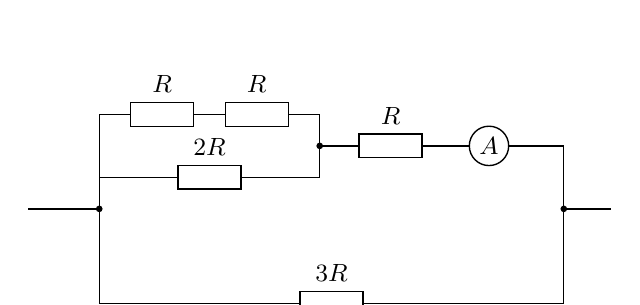
\begin{tikzpicture}[x=1cm,y=1cm,line width=0.5pt,>=Stealth,font=\small]
\draw (-0.6,1.2)--(0.3,1.2) (0.3,0)--(0.3,2.4) (6.2,0)--(6.2,2.0) (6.2,1.2)--(6.8,1.2);
\draw (0.3,2.4)--(0.7,2.4); \draw[fill=white] (0.7,2.25) rectangle (1.5,2.55); \node[above] at (1.1,2.55) {$R$};
\draw (1.5,2.4)--(1.9,2.4); \draw[fill=white] (1.9,2.25) rectangle (2.7,2.55); \node[above] at (2.3,2.55) {$R$}; \draw (2.7,2.4)--(3.1,2.4);
\draw (0.3,1.6)--(1.3,1.6); \draw[fill=white] (1.3,1.45) rectangle (2.1,1.75); \node[above] at (1.7,1.75) {$2R$}; \draw (2.1,1.6)--(3.1,1.6);
\draw (3.1,1.6)--(3.1,2.4); \draw (3.1,2.0)--(3.6,2.0); \draw[fill=white] (3.6,1.85) rectangle (4.4,2.15); \node[above] at (4.0,2.15) {$R$};
\draw (4.4,2.0)--(5.0,2.0); \draw[fill=white] (5.25,2.0) circle(0.25) node{$A$}; \draw (5.5,2.0)--(6.2,2.0);
\draw (0.3,0)--(2.85,0); \draw[fill=white] (2.85,-0.15) rectangle (3.65,0.15); \node[above] at (3.25,0.15) {$3R$}; \draw (3.65,0)--(6.2,0);
\fill (0.3,1.2) circle(1.2pt) (6.2,1.2) circle(1.2pt) (3.1,2.0) circle(1.2pt);
\end{tikzpicture}\par\smallskip
\opt{A}{15/2}
\opt{B}{15/4}
\opt{C}{15}
\opt{D}{30}
\end{minipage}\vspace{2pt}\par
\noindent\colorbox{gray!12}{\parbox{\dimexpr\linewidth-2\fboxsep}{\textbf{Javob: A) 15/2}}}\par\smallskip
\noindent\textit{Yechim.}\ Ampermetr yuqori tarmoqda: undan ötgan 1 A tok $R+R=2R$ va $2R$ dan iborat ikki parallel şoxga teng bölinadi — $2R$ rezistordan $0{,}5$ A ötadi.\par
\[Q=I^2\cdot2R\cdot t=0{,}25\cdot6\cdot5=7{,}5=\frac{15}{2}\ \text{J}.\]\par\medskip\hrule\medskip
\Needspace{10\baselineskip}\noindent\begin{minipage}{\linewidth}
\textbf{19.}\ Nuqtaviy zaryaddan 2 cm masofadagi nuqtada elektr maydon potensiali $-$2 V. Şu nuqtadagi maydon kuçlanganligini (V/m) toping.\par\smallskip
\opt{A}{50}
\opt{B}{100}
\opt{C}{10}
\opt{D}{400}
\end{minipage}\vspace{2pt}\par
\noindent\colorbox{gray!12}{\parbox{\dimexpr\linewidth-2\fboxsep}{\textbf{Javob: B) 100}}}\par\smallskip
\noindent\textit{Yechim.}\ Nuqtaviy zaryad uçun $|\varphi|=\frac{k|q|}{r}$, $E=\frac{k|q|}{r^2}=\frac{|\varphi|}{r}=\frac{2}{0{,}02}=100$ V/m.\par\par\medskip\hrule\medskip
\Needspace{10\baselineskip}\noindent\begin{minipage}{\linewidth}
\textbf{20.}\ Çeksiz uzunlikdagi özaro parallel ötkazgiçlarning har biridan mos ravişda 10 A va 20 A toklar ötmoqda. Agar bu ötkazgiçlarning har bir 2 metri 8$\cdot10^{-5}$ N kuç bilan özaro ta‘sirlaşsa, ötkazgiçlar orasidagi masofani toping (m).\par\smallskip
\opt{A}{2}
\opt{B}{0,5}
\opt{C}{1,5}
\opt{D}{1}
\end{minipage}\vspace{2pt}\par
\noindent\colorbox{gray!12}{\parbox{\dimexpr\linewidth-2\fboxsep}{\textbf{Javob: D) 1}}}\par\smallskip
\noindent\textit{Yechim.}\ Uzunligi $L$ bölgan qismga ta’sir kuçi\par
\[F=\frac{\mu_0I_1I_2L}{2\pi d}\ \Rightarrow\ d=\frac{2\cdot10^{-7}\cdot10\cdot20\cdot2}{8\cdot10^{-5}}=1\ \text{m}.\]\par\medskip\hrule\medskip
\Needspace{10\baselineskip}\noindent\begin{minipage}{\linewidth}
\textbf{21.}\ Zanjirning bir qismi ketma-ket ulangan pölat ($S_1$=0,48 mm$^{2}$, $l_1$=2 m) va nikelin ($S_2$=0,21 mm$^{2}$, $l_2$=1 m) simlardan tuzilgan. 0,6 A tok kuçini hosil qiliş uçun mazkur qismga qanday kuçlaniş qöyilişi lozim (V)? Pölat va nikelin simlarning soliştirma qarşiliklari mos ravişda $12\cdot10^{-8}$ $\Omega\cdot$m va $42\cdot10^{-8}$ $\Omega\cdot$m.\par\smallskip
\opt{A}{1,5}
\opt{B}{1}
\opt{C}{2}
\opt{D}{1,8}
\end{minipage}\vspace{2pt}\par
\noindent\colorbox{gray!12}{\parbox{\dimexpr\linewidth-2\fboxsep}{\textbf{Javob: A) 1,5}}}\par\smallskip
\noindent\textit{Yechim.}\ \[R_1=\frac{12\cdot10^{-8}\cdot2}{0{,}48\cdot10^{-6}}=0{,}5\ \Omega,\quad R_2=\frac{42\cdot10^{-8}\cdot1}{0{,}21\cdot10^{-6}}=2\ \Omega,\quad U=I(R_1+R_2)=0{,}6\cdot2{,}5=1{,}5\ \text{V}.\]\par\medskip\hrule\medskip
\Needspace{10\baselineskip}\noindent\begin{minipage}{\linewidth}
\textbf{22.}\ Özgaruvçan tok manbayiga aktiv qarşilik, induktiv ğaltak va kondensator ketma-ket ulangan. Aktiv qarşilikdagi kuçlaniş 2 V, kondensatordagi kuçlaniş 6 V. Agar zanjirdagi tok tebranişlari kuçlaniş tebranişlaridan faza böyiça $\dfrac{\pi}{4}$ orqada bölsa, induktiv ğaltakdagi kuçlanişni (V) aniqlang.\par\smallskip
\opt{A}{8}
\opt{B}{6}
\opt{C}{10}
\opt{D}{4}
\end{minipage}\vspace{2pt}\par
\noindent\colorbox{gray!12}{\parbox{\dimexpr\linewidth-2\fboxsep}{\textbf{Javob: A) 8}}}\par\smallskip
\noindent\textit{Yechim.}\ Tok kuçlanişdan $\pi/4$ orqada: $\mathrm{tg}\,\varphi=\frac{U_L-U_C}{U_R}=1$, $U_L=U_C+U_R=6+2=8$ V.\par\par\medskip\hrule\medskip
\Needspace{10\baselineskip}\noindent\begin{minipage}{\linewidth}
\textbf{23.}\ Qarşiligi 2 $\Omega$ bölgan rezistor kuçlanişi $u = 4\sqrt{2}\cos(\dfrac{\pi}{8}t)$ [V] qonun böyiça özgaradigan özgaruvçan tok manbayiga ulandi. $t$=10 s paytdagi tokning oniy quvvatini (W) aniqlang.\par\smallskip
\opt{A}{8}
\opt{B}{$16\sqrt{2}$}
\opt{C}{$8\sqrt{2}$}
\opt{D}{16}
\end{minipage}\vspace{2pt}\par
\noindent\colorbox{gray!12}{\parbox{\dimexpr\linewidth-2\fboxsep}{\textbf{Javob: A) 8}}}\par\smallskip
\noindent\textit{Yechim.}\ $u(10)=4\sqrt2\cos\frac{10\pi}{8}=4\sqrt2\cos225^\circ=-4$ V. Oniy quvvat $p=\frac{u^2}{R}=\frac{16}{2}=8$ W.\par\par\medskip\hrule\medskip
\Needspace{10\baselineskip}\noindent\begin{minipage}{\linewidth}
\textbf{24.}\ Siğimlari $C_1 = 3C_2 = 6C_3$ bölgan kondensatorlar özgarmas kuçlaniş manbayiga ketma-ket ulanib töliq zaryadlandi. Bunda $C_3$ siğimli kondensator $q$ zaryad töplagan bölsa, kalit $K$ ikkinçi holatga ötkazilsa $R$ qarşilikdan qança zaryad oqib ötadi?\par\smallskip
\noindent\hspace*{4mm}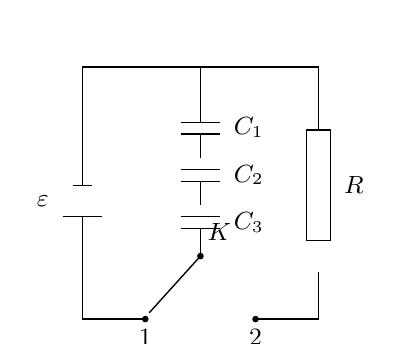
\begin{tikzpicture}[x=1cm,y=1cm,line width=0.5pt,>=Stealth,font=\small]
\draw (0,0.3)--(0,1.3) (0,1.7)--(0,3.2)--(3,3.2)--(3,2.4) (3,0.6)--(3,0);
\draw (-0.25,1.3)--(0.25,1.3) (-0.12,1.7)--(0.12,1.7); \node[left] at (-0.3,1.5) {$\varepsilon$};
\draw (1.5,3.2)--(1.5,2.8);
\foreach \y/\n in {2.5/1,1.9/2,1.3/3}{\draw (1.25,\y)--(1.75,\y) (1.25,\y-0.15)--(1.75,\y-0.15); \node[right] at (1.8,\y-0.07) {$C_\n$};}
\draw (1.5,2.5)--(1.5,2.8) (1.5,2.35)--(1.5,2.05) (1.5,1.75)--(1.5,1.45) (1.5,1.15)--(1.5,0.8);
\draw[fill=white] (3,2.0) rectangle ++(0,0); \draw[fill=white] (2.85,1.0) rectangle (3.15,2.4); \node[right] at (3.2,1.7) {$R$};
\draw (0,0.3)--(0,0)--(0.8,0) (2.2,0)--(3,0);
\fill (0.8,0) circle(1.2pt) node[below]{1}; \fill (2.2,0) circle(1.2pt) node[below]{2}; \fill (1.5,0.8) circle(1.2pt) node[left=3pt,above right=2pt]{$K$};
\draw (1.5,0.8)--(0.85,0.08);
\end{tikzpicture}\par\smallskip
\opt{A}{$q$}
\opt{B}{3$q$}
\opt{C}{9$q$}
\opt{D}{10$q$}
\end{minipage}\vspace{2pt}\par
\noindent\colorbox{gray!12}{\parbox{\dimexpr\linewidth-2\fboxsep}{\textbf{Javob: A) $q$}}}\par\smallskip
\noindent\textit{Yechim.}\ 1-holatda ketma-ket ulangan kondensatorlarning har biri bir xil $q$ zaryad oladi. 2-holatda kondensatorlar zanjiri manbadan uziladi va $R$ orqali razryadlanadi; ketma-ket zanjirdan $R$ orqali $q$ zaryad oqib ötadi.\par\par\medskip\hrule\medskip
\Needspace{10\baselineskip}\noindent\begin{minipage}{\linewidth}
\textbf{25.}\ Quyidagi magnit singdiruvçanligi berilgan moddalarning qaysi birlari ferromagnit? 1) $\mu$ = 800; 2) $\mu$ = 0,998; 3) $\mu$ = 0,999998; 4) $\mu$ = 1,00998; 5) $\mu$ = 998.\par\smallskip
\opt{A}{5}
\opt{B}{2, 3, 4}
\opt{C}{1, 5}
\opt{D}{2, 3}
\end{minipage}\vspace{2pt}\par
\noindent\colorbox{gray!12}{\parbox{\dimexpr\linewidth-2\fboxsep}{\textbf{Javob: C) 1, 5}}}\par\smallskip
\noindent\textit{Yechim.}\ Ferromagnitlarda $\mu\gg1$: $\mu=800$ va $\mu=998$ (1 va 5).\par\par\medskip\hrule\medskip
\Needspace{10\baselineskip}\noindent\begin{minipage}{\linewidth}
\textbf{26.}\ Yiğuvçi linza yordamida ekranda buyumning 2 marta kattalaşgan haqiqiy tasviri hosil qilindi. Buyum va tasvir orasidagi masofa 1,5 m bölsa, linzaning optik kuçini (dptr) aniqlang.\par\smallskip
\opt{A}{3}
\opt{B}{1/3}
\opt{C}{1/4}
\opt{D}{4}
\end{minipage}\vspace{2pt}\par
\noindent\colorbox{gray!12}{\parbox{\dimexpr\linewidth-2\fboxsep}{\textbf{Javob: A) 3}}}\par\smallskip
\noindent\textit{Yechim.}\ $\Gamma=2$, $d+f=1{,}5$ m: $d=0{,}5$ m, $f=1$ m.\par
\[D=\frac1d+\frac1f=2+1=3\ \text{dptr}.\]\par\medskip\hrule\medskip
\Needspace{10\baselineskip}\noindent\begin{minipage}{\linewidth}
\textbf{27.}\ Fokus masofasi 20 cm bölgan linzaning optik kuçi (dptr) qança?\par\smallskip
\opt{A}{10}
\opt{B}{$-$10}
\opt{C}{$-$5}
\opt{D}{5}
\end{minipage}\vspace{2pt}\par
\noindent\colorbox{gray!12}{\parbox{\dimexpr\linewidth-2\fboxsep}{\textbf{Javob: D) 5}}}\par\smallskip
\noindent\textit{Yechim.}\ Yiğuvçi linza: $D=1/F=1/0{,}2=5$ dptr.\par\par\medskip\hrule\medskip
\Needspace{10\baselineskip}\noindent\begin{minipage}{\linewidth}
\textbf{28.}\ Davri 2,3 $\mu$m bölgan difraksion panjaraga tölqin uzunligi 0,6 $\mu$m bölgan tölqin tik tuşmoqda. Ekranda hosil bölgan maksimumlar sonini aniqlang.\par\smallskip
\opt{A}{6}
\opt{B}{3}
\opt{C}{7}
\opt{D}{4}
\end{minipage}\vspace{2pt}\par
\noindent\colorbox{gray!12}{\parbox{\dimexpr\linewidth-2\fboxsep}{\textbf{Javob: C) 7}}}\par\smallskip
\noindent\textit{Yechim.}\ $k_{max}<\frac{d}{\lambda}=\frac{2{,}3}{0{,}6}\approx3{,}8$, ya’ni $k_{max}=3$. Maksimumlar soni $2\cdot3+1=7$.\par\par\medskip\hrule\medskip
\Needspace{10\baselineskip}\noindent\begin{minipage}{\linewidth}
\textbf{29.}\ Zarraning relyativistik impulsi klassik impulsidan $n$ marta katta bölsa, zarraning tezligini aniqlang. $c$ - yoruğlikning böşliqdagi tezligi.\par\smallskip
\opt{A}{$\dfrac{\sqrt{n^2-1}}{n}c$}
\opt{B}{$\dfrac{\sqrt{n^2+1}}{n}c$}
\opt{C}{$\dfrac{\sqrt{n^2-1}}{2n}c$}
\opt{D}{$\dfrac{\sqrt{n-1}}{n}c$}
\end{minipage}\vspace{2pt}\par
\noindent\colorbox{gray!12}{\parbox{\dimexpr\linewidth-2\fboxsep}{\textbf{Javob: A) $\dfrac{\sqrt{n^2-1}}{n}c$}}}\par\smallskip
\noindent\textit{Yechim.}\ $p=\frac{mv}{\sqrt{1-v^2/c^2}}=n\cdot mv$, ya’ni $\gamma=n$:\par
\[v=c\sqrt{1-\frac{1}{n^2}}=\frac{\sqrt{n^2-1}}{n}c.\]\par\medskip\hrule\medskip
\Needspace{10\baselineskip}\noindent\begin{minipage}{\linewidth}
\textbf{30.}\ Yadrodagi neytronlardan biri parçalansa, qanday hodisa sodir böladi?\par\smallskip
\opt{A}{$\gamma$-radioaktivlik}
\opt{B}{yadroda özgariş sodir bölmaydi}
\opt{C}{$\alpha$-radioaktivlik}
\opt{D}{$\beta$-radioaktivlik}
\end{minipage}\vspace{2pt}\par
\noindent\colorbox{gray!12}{\parbox{\dimexpr\linewidth-2\fboxsep}{\textbf{Javob: D) $\beta$-radioaktivlik}}}\par\smallskip
\noindent\textit{Yechim.}\ Neytronning yemirilişi $n\to p+e^-+\tilde\nu$ — bu $\beta$-radioaktivlik.\par\par\medskip\hrule\medskip
\Needspace{10\baselineskip}\noindent\begin{minipage}{\linewidth}
\textbf{31.}\ Radioaktiv preparatning radioaktiv yemiriliş doimiysi $4\cdot10^{-6}$ s$^{-1}$. Uning yarim yemiriliş davri (s) qanday? ln 2=0,7.\par\smallskip
\opt{A}{$3{,}5\cdot10^7$}
\opt{B}{$3{,}5\cdot10^6$}
\opt{C}{$1{,}75\cdot10^5$}
\opt{D}{$3{,}5\cdot10^4$}
\end{minipage}\vspace{2pt}\par
\noindent\colorbox{gray!12}{\parbox{\dimexpr\linewidth-2\fboxsep}{\textbf{Javob: C) $1{,}75\cdot10^5$}}}\par\smallskip
\noindent\textit{Yechim.}\ \[T=\frac{\ln2}{\lambda}=\frac{0{,}7}{4\cdot10^{-6}}=1{,}75\cdot10^5\ \text{s}.\]\par\medskip\hrule\medskip
\Needspace{10\baselineskip}\noindent\begin{minipage}{\linewidth}
\textbf{32.}\ Jism 80 m öngga, keyin esa 30 m qarama-qarşi tomonga yuridi. Jismning köçisini (m) aniqlang.\par\smallskip
\opt{A}{50}
\opt{B}{25}
\opt{C}{75}
\opt{D}{100}
\end{minipage}\vspace{2pt}\par
\noindent\colorbox{gray!12}{\parbox{\dimexpr\linewidth-2\fboxsep}{\textbf{Javob: A) 50}}}\par\smallskip
\noindent\textit{Yechim.}\ Köçiş $80-30=50$ m.\par\par\medskip\hrule\medskip
\newpage\noindent\textbf{33–35.}\ Bir jinsli magnit maydonda ($B=0,5$ T, maydon çiziqlari rasm tekisligiga tik) uzunligi $l=0,4$ m bölgan ötkazgiç sterjen tezlikka tik yönalişda $v=5$ m/s tezlik bilan siljiydi. Relslarning qarşiligi nolga teng, zanjirning qarşiligi $R=0,5\ \Omega$.\par\medskip
\begin{center}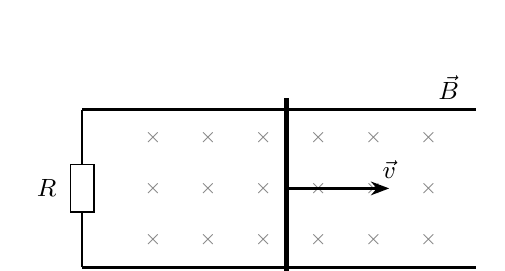
\begin{tikzpicture}[x=1cm,y=1cm,line width=0.5pt,>=Stealth,font=\small]
\draw[line width=1pt] (0,0)--(5.0,0) (0,2)--(5.0,2); \draw (0,0)--(0,0.7) (0,1.3)--(0,2); \draw[fill=white] (-0.15,0.7) rectangle (0.15,1.3); \node[left] at (-0.2,1) {$R$};
\foreach \x in {0.9,1.6,2.3,3.0,3.7,4.4}{\foreach \y in {0.35,1.0,1.65}{\node[font=\scriptsize,gray] at (\x,\y) {$\times$};}}
\draw[line width=1.8pt] (2.6,-0.15)--(2.6,2.15); \draw[->,thick] (2.6,1.0)--(3.9,1.0) node[above]{$\vec v$}; \node[above right] at (4.4,2.0) {$\vec B$};
\end{tikzpicture}\end{center}
\noindent\textbf{33.}\ Sterjenda induksiyalangan EYuKni (V) toping.\par
\noindent\textbf{34.}\ Zanjirdagi tok kuçini (A) toping.\par
\noindent\textbf{35.}\ Sterjenga ta’sir qiluvçi Amper kuçini (N) toping.\par
\noindent Variantlar: A) 0,4;\quad B) 0,5;\quad C) 0,8;\quad D) 1;\quad E) 2;\quad F) 4\par\smallskip
\noindent\colorbox{gray!12}{\parbox{\dimexpr\linewidth-2\fboxsep}{\textbf{Javob: 33--D) 1; 34--E) 2; 35--A) 0,4}}}\par\smallskip
\noindent\textit{Yechim.}\ \[\mathcal E=Blv=0{,}5\cdot0{,}4\cdot5=1\ \text{V},\qquad I=\frac{\mathcal E}{R}=2\ \text{A},\qquad F=BIl=0{,}5\cdot2\cdot0{,}4=0{,}4\ \text{N}.\]\par\medskip\hrule\medskip
\Needspace{12\baselineskip}\noindent\textbf{36.}\ Yuzasi 2 m$^2$, qalinligi 30 cm bölgan muz parçasi suvda suzib yuribdi. $\rho_{muz}=900$ kg/m$^3$, $\rho_{suv}=1000$ kg/m$^3$.\par
\noindent\hspace*{4mm}a)\ Muz parçasining suvdan çiqib turgan qismi balandligini (cm) toping.\par
\noindent\hspace*{4mm}b)\ Muz parçasi töliq botib ketmasligi uçun uning ustiga çiqişi mumkin bölgan odamning eng katta massasini (kg) toping.\par
\noindent\colorbox{gray!12}{\parbox{\dimexpr\linewidth-2\fboxsep}{\textbf{Javob: a)\ 3;\quad b)\ 60}}}\par\smallskip
\noindent\textit{Yechim.}\ Suziş şarti: botgan qism $h_b=\frac{\rho_m}{\rho_s}h=27$ cm, suvdan çiqib turgan qism $30-27=3$ cm. Töliq botiş uçun qöşimça massa\par
\[M=\rho_sS\cdot0{,}03=1000\cdot2\cdot0{,}03=60\ \text{kg}.\]\par\medskip\hrule\medskip
\Needspace{12\baselineskip}\noindent\textbf{37.}\ Jismning koordinatasi vaqtga boğliq ravişda $x=5+4t-t^2$ (m) qonun böyiça özgaradi.\par
\noindent\hspace*{4mm}a)\ $t=3$ s paytdagi jism tezligini (m/s) toping.\par
\noindent\hspace*{4mm}b)\ Dastlabki 3 s davomida jism bosib ötgan yölni (m) toping.\par
\noindent\colorbox{gray!12}{\parbox{\dimexpr\linewidth-2\fboxsep}{\textbf{Javob: a)\ -2;\quad b)\ 5}}}\par\smallskip
\noindent\textit{Yechim.}\ $v=x'=4-2t$, $v(3)=-2$ m/s. Jism $t=2$ s da töxtab orqaga qaytadi: $x(0)=5$, $x(2)=9$, $x(3)=8$ m. Yöl $4+1=5$ m.\par\par\medskip\hrule\medskip
\Needspace{12\baselineskip}\noindent\textbf{38.}\ Massasi 4 kg bölgan miltiqdan massasi 10 g bölgan öq 600 m/s tezlik bilan otildi.\par
\noindent\hspace*{4mm}a)\ Miltiqning orqaga tepiş tezligini (m/s) toping.\par
\noindent\hspace*{4mm}b)\ Miltiqning orqaga tepiş kinetik energiyasini (J) toping.\par
\noindent\colorbox{gray!12}{\parbox{\dimexpr\linewidth-2\fboxsep}{\textbf{Javob: a)\ 1,5;\quad b)\ 4,5}}}\par\smallskip
\noindent\textit{Yechim.}\ Impulsning saqlaniş qonuni: $Mu=mv$, $u=\frac{0{,}01\cdot600}{4}=1{,}5$ m/s. $E_k=\frac{4\cdot1{,}5^2}{2}=4{,}5$ J.\par\par\medskip\hrule\medskip
\Needspace{12\baselineskip}\noindent\textbf{39.}\ Issiqlik dvigatelining FIK 25\%, foydali quvvati 40 kW. Yoqilğining soliştirma yoniş issiqligi 40 MJ/kg.\par
\noindent\hspace*{4mm}a)\ Dvigatelga yoqilği yonişidan 1 s da beriladigan issiqlik miqdorini (kJ) toping.\par
\noindent\hspace*{4mm}b)\ Dvigatel 1 soatda qança (kg) yoqilği sarflaydi?\par
\noindent\colorbox{gray!12}{\parbox{\dimexpr\linewidth-2\fboxsep}{\textbf{Javob: a)\ 160;\quad b)\ 14,4}}}\par\smallskip
\noindent\textit{Yechim.}\ 1 s da beriladigan issiqlik $Q=\frac{P}{\eta}=\frac{40}{0{,}25}=160$ kJ. 1 soatda $160\cdot3600=576$ MJ, yoqilği massasi $576/40=14{,}4$ kg.\par\par\medskip\hrule\medskip
\Needspace{12\baselineskip}\noindent\textbf{40.}\ $-10$ $^\circ$C temperaturali 2 kg muzni 0 $^\circ$C dagi suvga aylantiriş kerak. $c_{muz}=2100$ J/(kg$\cdot$K), $\lambda_{muz}=330$ kJ/kg.\par
\noindent\hspace*{4mm}a)\ Muzni eriş temperaturasigaça isitiş uçun kerak bölgan issiqlik miqdorini (kJ) toping.\par
\noindent\hspace*{4mm}b)\ Butun jarayon uçun kerak bölgan issiqlik miqdorini (kJ) toping.\par
\noindent\colorbox{gray!12}{\parbox{\dimexpr\linewidth-2\fboxsep}{\textbf{Javob: a)\ 42;\quad b)\ 702}}}\par\smallskip
\noindent\textit{Yechim.}\ $Q_1=c_mm\Delta t=2100\cdot2\cdot10=42$ kJ; eritiş $Q_2=\lambda m=660$ kJ. Jami $702$ kJ.\par\par\medskip\hrule\medskip
\Needspace{12\baselineskip}\noindent\textbf{41.}\ Tebraniş konturi induktivligi 1 mH bölgan ğaltak va siğimi 1 nF bölgan kondensatordan iborat. $\pi=3{,}14$, $c=3\cdot10^8$ m/s.\par
\noindent\hspace*{4mm}a)\ Konturdagi erkin elektromagnit tebranişlar davrini ($\mu$s) toping.\par
\noindent\hspace*{4mm}b)\ Kontur nurlaydigan elektromagnit tölqin uzunligini (m) toping.\par
\noindent\colorbox{gray!12}{\parbox{\dimexpr\linewidth-2\fboxsep}{\textbf{Javob: a)\ 6,28;\quad b)\ 1884}}}\par\smallskip
\noindent\textit{Yechim.}\ \[T=2\pi\sqrt{LC}=6{,}28\sqrt{10^{-3}\cdot10^{-9}}=6{,}28\cdot10^{-6}\ \text{s},\qquad \lambda=cT=3\cdot10^8\cdot6{,}28\cdot10^{-6}=1884\ \text{m}.\]\par\medskip\hrule\medskip
\Needspace{12\baselineskip}\noindent\textbf{42.}\ $q$ va $4q$ musbat nuqtaviy zaryadlar bir-biridan 30 cm masofada mahkamlangan. Ular orasiga uçinçi nuqtaviy zaryad joylaştirildi.\par
\noindent\hspace*{4mm}a)\ Uçinçi zaryad muvozanatda bölişi uçun u $q$ zaryaddan qanday masofada (cm) joylaşişi kerak?\par
\noindent\hspace*{4mm}b)\ Uçala zaryad ham muvozanatda bölişi uçun uçinçi zaryadning $q$ ga nisbati $q_3/q$ qanday bölişi kerak (önli kasrda, işorasi bilan)?\par
\noindent\colorbox{gray!12}{\parbox{\dimexpr\linewidth-2\fboxsep}{\textbf{Javob: a)\ 10;\quad b)\ -0,444}}}\par\smallskip
\noindent\textit{Yechim.}\ Uçinçi zaryadga ta’sir kuçlari teng: $\frac{q}{x^2}=\frac{4q}{(0{,}3-x)^2}$, $0{,}3-x=2x$, $x=0{,}1$ m $=10$ cm. $q$ zaryadning muvozanati: $\frac{kqq_3}{0{,}1^2}+\frac{kq\cdot4q}{0{,}3^2}=0$,\par
\[q_3=-4q\cdot\frac{0{,}01}{0{,}09}=-\frac49q\approx-0{,}444q.\]\par\medskip\hrule\medskip
\Needspace{12\baselineskip}\noindent\textbf{43.}\ Vakuumdagi tölqin uzunligi 600 nm bölgan yoruğlik suvga ötdi. $n_{suv}=4/3$, $c=3\cdot10^8$ m/s.\par
\noindent\hspace*{4mm}a)\ Yoruğlik çastotasini ($10^{14}$ Hz) toping.\par
\noindent\hspace*{4mm}b)\ Yoruğlikning suvdagi tölqin uzunligini (nm) toping.\par
\noindent\colorbox{gray!12}{\parbox{\dimexpr\linewidth-2\fboxsep}{\textbf{Javob: a)\ 5;\quad b)\ 450}}}\par\smallskip
\noindent\textit{Yechim.}\ Çastota muhitga boğliq emas: $\nu=\frac{c}{\lambda}=\frac{3\cdot10^8}{6\cdot10^{-7}}=5\cdot10^{14}$ Hz. Suvda $\lambda'=\lambda/n=600\cdot\frac34=450$ nm.\par\par\medskip\hrule\medskip
\Needspace{12\baselineskip}\noindent\textbf{44.}\ Uzoqni yaxşi köra olmaydigan odamning aniq körişining eng uzoq nuqtasi 50 cm masofada. Yaqindan yaxşi köra olmaydigan boşqa odamning aniq körişining eng yaqin nuqtasi 50 cm masofada. Eng yaxşi köriş masofasi 25 cm.\par
\noindent\hspace*{4mm}a)\ Birinçi odamga kerak bölgan közoynak optik kuçini (dptr) toping.\par
\noindent\hspace*{4mm}b)\ Ikkinçi odamga kerak bölgan közoynak optik kuçini (dptr) toping.\par
\noindent\colorbox{gray!12}{\parbox{\dimexpr\linewidth-2\fboxsep}{\textbf{Javob: a)\ -2;\quad b)\ 2}}}\par\smallskip
\noindent\textit{Yechim.}\ Yaqindan köruvçi (miop) uçun soçuvçi közoynak: $D=-\frac{1}{0{,}5}=-2$ dptr. Uzoqdan köruvçi uçun buyum 25 cm da, tasvir 50 cm da (mavhum):\par
\[D=\frac{1}{0{,}25}-\frac{1}{0{,}5}=2\ \text{dptr}.\]\par\medskip\hrule\medskip
\Needspace{12\baselineskip}\noindent\textbf{45.}\ $^{235}$U yadrosining bitta bölinişida 200 MeV energiya ajraladi. $N_A=6{,}02\cdot10^{23}$ mol$^{-1}$, 1 MeV $=1{,}6\cdot10^{-13}$ J.\par
\noindent\hspace*{4mm}a)\ 1 g uran-235 dagi yadrolar sonini ($10^{21}$) toping.\par
\noindent\hspace*{4mm}b)\ 1 g uran-235 töliq bölinganda ajraladigan energiyani ($10^{10}$ J) toping.\par
\noindent\colorbox{gray!12}{\parbox{\dimexpr\linewidth-2\fboxsep}{\textbf{Javob: a)\ 2,56;\quad b)\ 8,2}}}\par\smallskip
\noindent\textit{Yechim.}\ \[N=\frac{m}{M}N_A=\frac{1}{235}\cdot6{,}02\cdot10^{23}\approx2{,}56\cdot10^{21},\qquad E=N\cdot200\cdot1{,}6\cdot10^{-13}\approx8{,}2\cdot10^{10}\ \text{J}.\]\par\medskip\hrule\medskip
\end{document}